\label{binary}

Основная идея алгоритма с несмещенныи бинарными операторами заключается в следующих двух этапах: формирование независимых уникальных строк без использования операторов 
с помощью примитивных пошаговых пеобразований и формирование всего оставшегося множества поиска, стараясь минимизировать количество повторений. 

Рассмотрим первый этап: создание множества уникальных строк.

Введем следующее: пусть ${I_0}^1 = \{1,\ldots, n\}$ - множество индексов в искомом экземпляре, поданном на вход задаче. 

Каждый этап выглядит следующим образом: 
\begin{align*}
& L_i = \langle \mathcal{I}_i = \{{\mathcal{I}_{i}}^{1},....{\mathcal{I}_{i}}^{k};\}; \:\: \textrm{где}  \cupdot_{a = 1..k_i} {I_i}^a = \{ 1..n \}; \\
& S_i = \{ {S_i}^1, ... {S_i}^{m_i}, \}, \textrm{где}  \\ 
&{s_i}^j = b_1..b_{k_i}, b_k = \{ 0..1  \}  \Longleftrightarrow b_1 \textrm{ на индексах } {I_{i}}^1, \\ & \:\:\:\:\:\:\:\:\:\:\:\:\:\:\:\:\:\:\:\:\:\:\:\:\:\:\:\:\:\:\:\:\:\:\:\:\:\:\:\:\:\:\:\:\:\:\:\:\:\:\:\:\:\:\:\: b_e \textrm{ на индексах } {I_{i}}^e\\
 \rangle
\end{align*}

Таким образом, самый первый уровень будет выглядеть так: 
$$L_0 = \langle \{\{ 1...n \}\}, \{0\} \rangle.$$

Каждый последующий уровень $L_i$ можно получить двумя способами: 
\begin{itemize}
   \item Разделить одно из множеств индексов пополам: $ \mathcal{{I}_i}^j \to \{\mathcal{{I}_{i+1}}^j, \mathcal{{I}_{i+1}}^{k_i+1}\} $, где $j \in [1..k_i]$;
   \item Преобразование строк с помощью операций, не разрезающих множества индексов.
\end{itemize}

При разделении множества индексов, уже имеющиеся строки преобразуются удваиванием бита, находящегося на позиции, множество индексов которого разделилось.
Таким образом гарантируется, что следующая полученная строка будет уникальна.

К неразделяющим множества индексов операциям относятся следующие оперции, которые можно применять попарно ко всем полученным векторам: 
переворот несовпадающих бит, переворот совпадающих бит, поворот совпадающих и несовпадающих бит. 
Нетрудно заметить, что данные операции являются несмещенными, так как не ориентируются на положение бита, а только на совпадение в этой же позиции с битом второго вектора. 

Таким образом генерируются маски последуюших строк. 

\begin{example}
Пример генерации строк для вектора размера $n = 6$ \\
    I = \{1, 2, 3,4,5,6\} \:\: S = \{0\} \\
    I = \{1, 2, 3,4,5,6\}  \:\: S = \{0, 1\} \\
    I = \{1, 2, 3\}, \{4,5,6\} \:\: S = \{00, 11\} \\
    I = \{1, 2, 3\}, \{4,5,6\} \:\: S = \{00, 11, 01, 10\} \\
    I = \{1, 2\}, \{3\}, \{4,5,6\} \:\: S = \{000, 111, 001, 110\} \\
    I = \{1, 2\}, \{3\}, \{4,5,6\} \:\: S = \{000, 111, 001, 110, 011, 100\} \\
    ...
\end{example}

В силу перечисленных выше изменений векторов, из полученных масок и индексов генерируется некоторое число уникальных строк. 
Так как таким путем нельзя получить полное множество поиска, оставшиеся строки генерируются следующим образом:  

\begin{algorithm}[!h]
\caption{Black-box алгоритм в несмещенной модели}\label{lst1}
\begin{algorithmic}
		\For{$t = S_1,S_2,S_3,...,S_\phi$ }
	    \State choose $i \in [1 : \phi] $
	    \State choose $j \in [1 : \phi] $
	    \State $e \leftarrow$ same bits in $\{S_i, S_j\}$
	    \State $d \leftarrow$ different bits in $\{S_i, S_j\}$
	    \State choose $k \in [1 : e] $
	    \State choose $l \in [1 : e] $
	    \State add to $T_{ijkl}$ - множество строк, генерируемых из $S_i$ и $S_j$ путем инвертирования k совпадающих и l различающихся бит в $S_i$
		\EndFor
\end{algorithmic}
\end{algorithm}

Таким образом генерируется множество конструкций, содержащих $T_{ijkl}$:   $\mathbb{T} = \{ T_{ijkl} \}$.
    
    \begin{math}
        \mathbb{T'} \subseteq \mathbb{T} : 
                   \left\{  
           \begin{array}{rcl}  
            \forall t, u \in \mathbb{T'} \quad t \cap u = \varnothing \\  
              \cup = {\{0, 1 \}}^n \setminus \{S_1...S_{\phi}\} \\  
           \end{array}   
           \right.
    \end{math}


Таким образом, мы получаем область поиска с некоторыми повторами, что немного, но улучшает работу. С увеличением длины подаваемого на вход вектора, увеличивается количество повторов.
На рисунке~\ref{fig1} показано распределение множества $T'$ для $n = 6$. При этом размер множества составлял 4097 строк.

\begin{figure}[H]
\centering
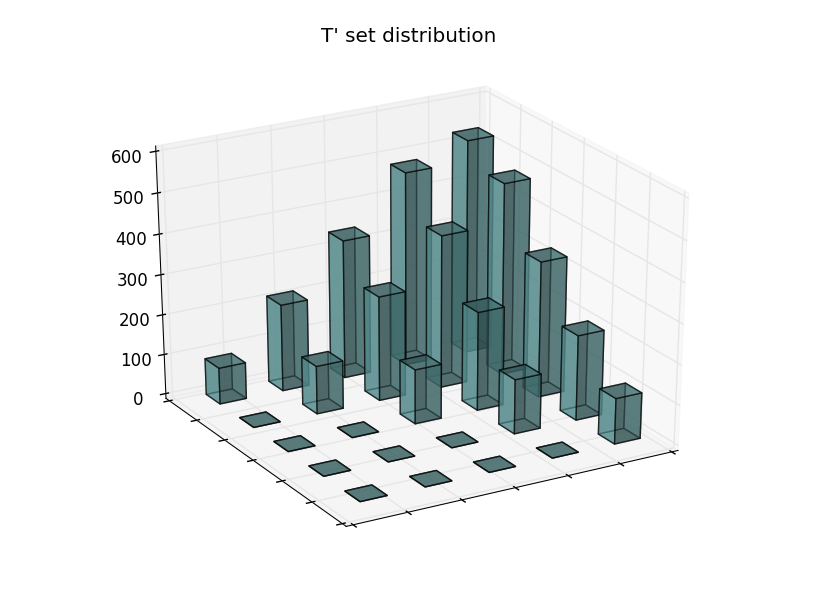
\includegraphics[height=10cm]{pic/fig6_n.png}
\caption{Распределение для n = 6}\label{fig1}
\end{figure}

Для улучшения результатов, применим к получившемся множествам некоторые преобразования. Сравним некоторые множества $T_{ijkl}$ между собой на наличие повторяющихся строк следующим образом: 

\begin{algorithm}[H]
\caption{Фильтрация повторяющихся множеств}\label{lst1}
\begin{algorithmic}
        \State Создаем неориентированный граф, вершины которого - множества $T_{ijkl}$ 
        \For{$i = 0, 1, \ldots, \mathbb{T}.same$}
	        \For{$j = 0, 1, \ldots, \mathbb{T}.diff$}
    	        \State Если между двумя множествами нет совпадающих строк, то соединяем данные вершины ребром.   
	        \EndFor
	    \EndFor
	    \State Дальнейшая задача сводится к поиску максимальной клики в графе.
\end{algorithmic}
\end{algorithm} 

По результатам работы алгоритма были рассмотрены два варианта действий. 
Рассмотрим несколько максимальных полученных клик, множества которых покрывают все пространство поиска. Экспериментально было установлено, что в результате нахождения клик
было отброшено достаточно большое количество повторов и итоговое отфильтрованное множество содержало и меньше векторов, и меньше повторов. 
Рассматривалось распределение для $n = 6$. В результате перебора всех пар значений было получено 4097 строк. По результатам фильтрации и поиска непересекающихся множеств осталось 306 векторов.
На рисунке~\ref{fig2} показано распределение при объединении двух клик. 

\begin{figure}[H]
\centering
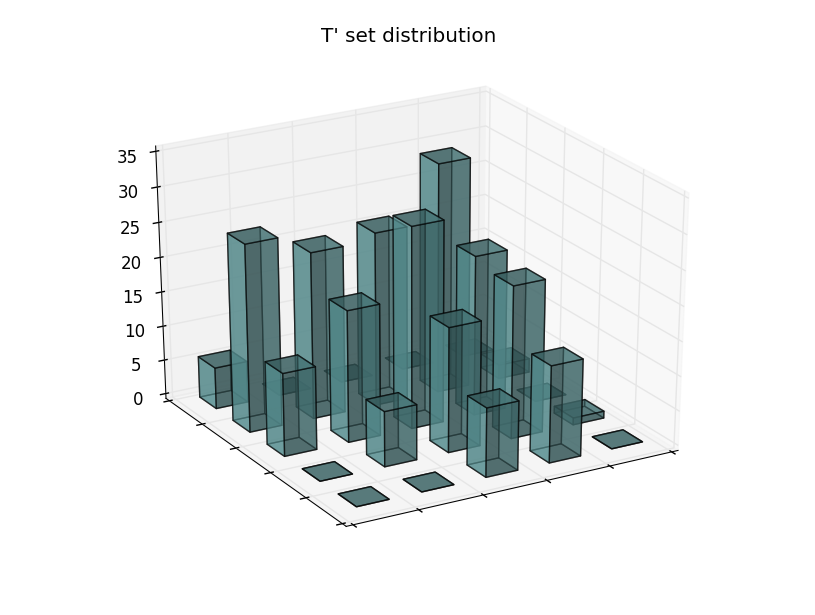
\includegraphics[height=10cm]{pic/fig6_mod2.png}
\caption{Выборка непересекающихся множеств для $n = 6$, подход 1}\label{fig2}
\end{figure}

Второй подход заключается

В результате выполнения алгоритма, гарантируется, что на выходе получится множество строк без повторов. 
При объединении полученного множества $T$ и получившихся на первом этапе строк, итоговое множетсво не превышает $2\cdot2^n$. 
Таким образом получается следующее распределение для $n = 6$, при этом размер множества составлял 124 строки. 

\begin{figure}[H]
\centering
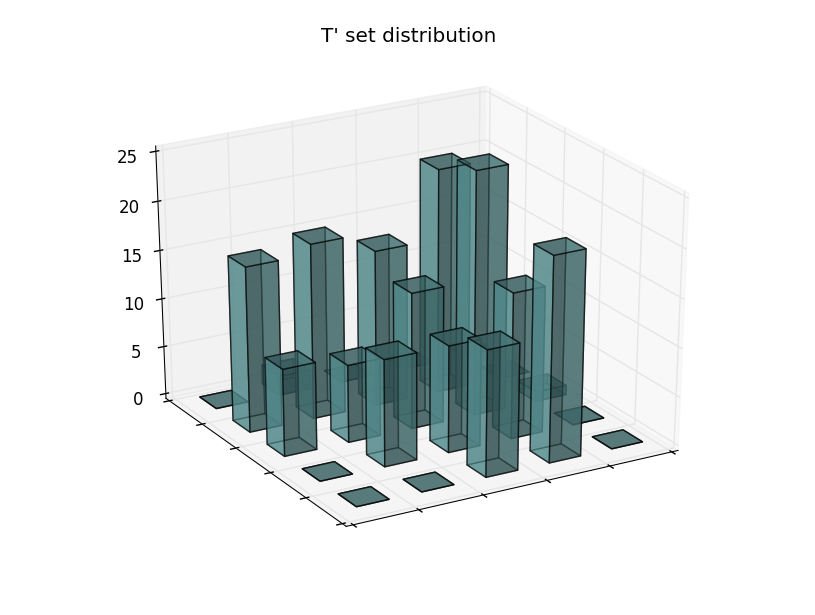
\includegraphics[height=10cm]{pic/fig6_mod3.png}
\caption{Выборка непересекающихся множеств для n = 6, подход 2}\label{fig2}
\end{figure}

В результате вызыва алгоритма для особей маленьких размеров, было замечено, что размер множества с повторами от увеличения размера особи растет экспоненциально. В таблице представлены результаты запуска для некоторых векторов:

\begin{table}[!h]
\caption{Результаты работы алгоритма с бинарными операторами}\label{tab3:apx}
\centering
\begin{tabu}{|*{6}{X[c]|}}\hline
n & 3 & 4 & 5 & 6 & 7  \\
\hline
set size & 8 & 16 & 32 & 64 & 128 \\
\hline
{T' size} & 64 & 256 & 1024 & 4096 & 16384  \\
\hline
{mod(T') size} & 11 & 36 & 73 & 144 & 302  \\
\hline
\end{tabu}
\end{table}

Ниже на рисунке~\ref{fig3} приводится диаграмма по количеству полученных совпавших строк и количеству оставшихся после модификации (берется лучшее значение).

\begin{figure}[H]
\centering
\caption{Выборка непересекающихся множеств для $n = 6$, подход 2}\label{fig3}
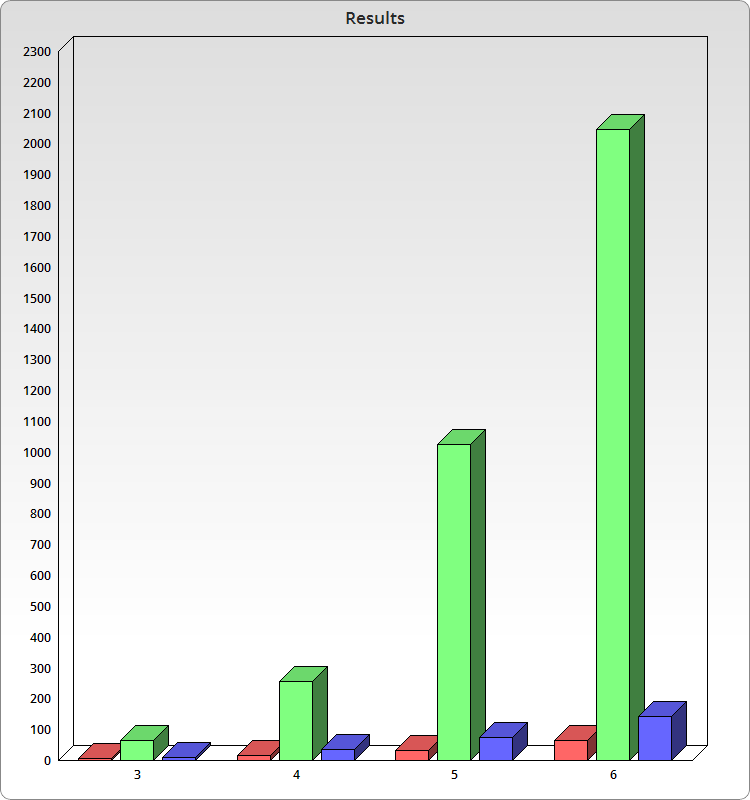
\includegraphics[height=10cm]{pic/res_bin.png}
\end{figure}
